\chapter{Osnove metamaterialov}\label{sec:osnove_metamaterialov}

    Metamateriali (MM) so umetno strukturirani kompoziti, ki so zgrajeni iz periodično razporejenih gradnikov, ki ne le da izboljšujejo lastnosti osnovnega materiala, temveč dajejo tudi različne funkcionalnosti, kot so negativni lomni količnik, negativna masna gostota, negativno Poissonovo razmerje, negativna dielektričnost, negativna permeabilnost, negativna stisljivost, negativni koeficienta toplotnega raztezka in tako dalje. Lastnosti metamaterialov so spremenjene tako, da presegajo lastnosti, ki jih najdemo v naravi. Tam najdemo celične strukture, kot so votlosti v pluti ali kosteh, vendar tam ne gre za periodične strukture, vendar le naključno razporejene nehomogenosti materiala. Pravi MM imajo periodično razporejene reprezentativne osnovne celice (ROC). Povzeto po \cite{Dalela2022} in \cite{Ji2021}. 
    
    Prvi MM so bili uvedeni na elektromagnetnem področju, pozneje pa je bil koncept metamaterialov razširjen tudi na optiko, akustiko in navsezadnje tudi na mehaniko trdnih teles kot vibroizolator z negativno togostjo. Klasifikacijo MM lahko vidimo na sliki  \ref{fig:klasifikacija metamaterialov}. 
    
    \begin{figure}[!hb]
            \centering
            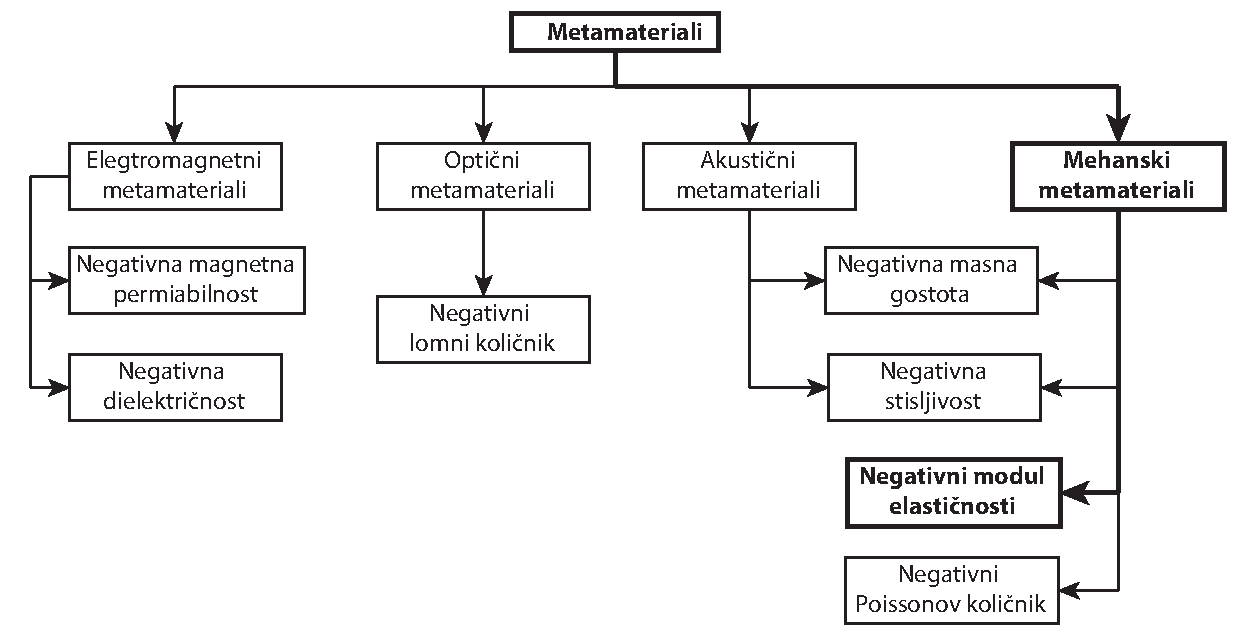
\includegraphics[width=\linewidth]{Magisterski praktikum/slike/teorija/klasifikacija_metamaterialov.pdf}
            \caption{Klasifikacija metamaterialov.}\label{fig:klasifikacija metamaterialov}
    \end{figure}

    \newpage
    
    Mehanski in akustični metamateriali med drugim vključujejo celične metamateriale, pomožne metamateriale z negativnim Poissonovim količnikom, pentamode metamateriale z znatno večjim stisljivostnim modulom kot strižnim modulom, metamaterialne strukture na osnovi origamija in materiale z lastnostjo pasovne vrzeli. Te vsi so obetavni za nadzor vibracij in zvoka. V našem primeru uporabimo koncept metamateriala z lastnostjo pasovne vrzeli. 
    
    Mehanske metamateriale za vibroizolacijo lahko razvijemo tako, da v glavni strukturi naredimo nekaj mehanskih podenot ali reprezentativnih osnovnih celic (ROC), tako da lahko mehanski valovi, ki se prenašajo v gradnikih, resonirajo s podenotami strukture. MM tako izraža lastnosti pasovno zavrnitvenega filtra (PZF), kar pomeni, da v določenem frekvenčnem območju MM ne dopušča, ali vsaj bistveno zmanjša širjenje valovanja. Naš cilj je torej razviti nov model MM za izboljšanje položaja in pasovne širine zavrnitvenega pasu. Obstajata dva pristopa za preučevanje značilnosti zapornih pasov: Braggovo sipanje (\textit{ang. Bragg scattering}) in princip lokalnih resonanc. 
    
    Kadar je širjenje valovanja odvisno le od periodične razporeditve in velikosti ROC v mediju, se te imenujejo fononski kristali. Pri fononskih kristalih je ena od najpomembnejših značilnosti učinek Braggovega sipanja, ki jih povzroči destruktivna interferenca prihajajočih in odbitih valov. Učinek Braggovega sipanja je omejen z velikostjo konstante mreže podstruktur. Na splošno so mere ROC v MM običajno manjše od valovne dolžine lastnosti, na katero vplivajo. Za dušenje visokih frekvenc posledično potrebujemo majhne, za nizkofrekvenčne PZF pa bi potrebovali zelo velike ROC, kar je iz vidika izdelave metamateriala nepraktično. 
    
    Rešitev omejitve velikosti je učinek lokalne resonance. Ta povzroči nizkofrekvenčno pasovno vrzel z mrežno konstanto, ki je za več redov manjša od valovne dolžine razširjajočih se valov. Fenomen pasovne vrzeli in pasovne širine, ki nastane zaradi lokalne resonance, je odvisen od geometrijskih parametrov in materialnih lastnosti resonatorjev; ni odvisen od periodičnosti in razporeditve ROC. Običajno to pomeni, da je vsaka ROC sistem masa-vzmet, katere lastna frekvenca $\omega_0=\sqrt{k/m}$ je odvisna od togosti $k$ njene interne vzmeti in mase $m$ (poglavje \ref{sec:dvomasni_dušilec_nihanj}). Za nizkofrekvenčno izolacijo vibracij mora biti bodisi masa zelo velika bodisi togost majhna. Resonator je omejen z veliko maso ali majhno togostjo. Da bi premagali to omejitev lahko v ROC z obstoječo pozitivno togostjo (PT) dodamo negativno togost (NT) in tako linearno togost spremenimo v nelinearno. Tako dosežemo kvazi ničelno togost (KNT), kar omogoča PZF zelo nizkih frekvenc.  
    
    V sledečem poglavju \ref{sec:ROC_statika} matematično zasnujemo ROC z KNT preko enačb strukturne statike in stabilnosti.
    
    
\newpage
\chapter{Analitična izpeljava ROC}\label{sec:ROC_statika}

    V sledečem poglavju zasnujemo reprezentativno osnovno celico (ROC) z visoko statično in nizko dinamično togostjo (VSND), ki ima lastnost kvazi ničelne togosti (KNT) (\cite{dalela2022design, fan2020design, cai2020design} ). Za primer sistema z eno prostostno stopnjo, sposobnost pasivnega dušenja pri nizkih frekvencah zavisi od sposobnosti zagotoviti majhno togost ali veliko maso sistema. Ker je masa najpogosteje nespremenljiva, želimo čim manjšo togost, kar pa pomeni nesposobnost prenašanja večjih statičnih obremenitev. Torej želimo vibroizolacijo, kjer prvotno statično obremenitev prevzame visoka togost, dinamične obremenitve pa se srečajo z nizko togostjo. VSND togost dosežemo z nelinearno vzmetjo s KNT, ki jo dobimo tako, da pozitivni togosti nasprotujemo z negativno togostjo. Najbolj tipični KNT vibroizolator \cite{lan2014design} je sestavljen iz treh vzmeti - iz vertikalne vzmeti, ki nosi statične obremenitve na tlak in zagotavlja pozitivno togost $k_p$ ter dveh paralelno vezanih horizontalnih vzmeti. Te nudijo negativno togost $k_n$, ki izniči pozitivno togost navpične vzmeti (slika \ref{fig:vzmetna_KNT_ROC}). Za našo aplikacijo metamateriala narejenega z aditivno tehnologijo, kjer je ROC zvezna struktura, moramo vzmeti nadomestiti s strukturam prijazni metodi izdelave. Pozitivno togost lahko tvorimo z navpičnimi ukrivljenimi nosilci in negativno togost z ukrivljenimi horizontalnimi nosilci, kjer imamo ob obremenitvi preskok sistema. Nosilci so zaprti znotraj bolj togega okvirja (slika \ref{fig:3D tiskana_KNT_ROC}).
    \begin{figure}[!htb]
        \centering
        \begin{subfigure}{.4\textwidth}
            \centering
            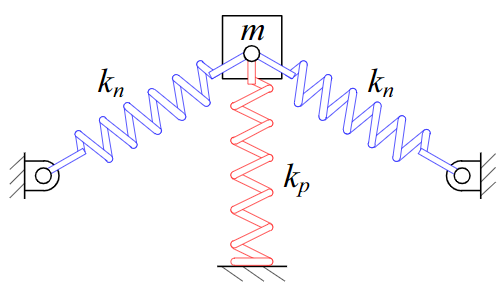
\includegraphics[trim=0 0 -2cm 0, clip, width=\linewidth]{Magisterski praktikum/slike/teorija/vzmetna_KNT_ROC.png}
            \caption{}
            \label{fig:vzmetna_KNT_ROC}
        \end{subfigure}%
        \begin{subfigure}{.3\textwidth}
            \centering
            
\includegraphics[trim=-5cm 0 0 0, clip, width=\linewidth]{Magisterski praktikum/slike/teorija/3D tiskana_KNT_ROC.png}
            \caption{}
            \label{fig:3D tiskana_KNT_ROC}
        \end{subfigure}%
        \caption{(a) Vzmetni KNT mehanizem in (b) 3D tiskana KNT ROC.}
    \end{figure}
    
    V sledečem poglavju analitično z enačbami, statike, trdnosti in stabilnosti zasnujemo KNT ROC. Sprva izpeljemo enačbe za navpične nosilce za pozitivno togost $k_p$ in nato enačbe za poševne nosilce z negativno togostjo $k_n$. Z glavnim pogojem KNT  povežemo vse nosilce skupaj v ROC z KNT: 
    \begin{align}\label{eq:pogoh_KNT}
        \frac{1}{2} (2 k_p +  k_n) = 0 \,.
    \end{align}
    
    
    \newpage
    \section{Izpeljava elementa s pozitivno togostjo}\label{sec:Izpeljava_elementa_s_pozitivno_togostjo}
    
        Pozitivni element je sestavljen iz simetričnih ukrivljenih nosilcev z togostjo $k_p$ in ga obravnavamo kot en sam Eulerjev-Bernoullijev nosilec, pri čemer upoštevamo le notranji moment (slika \ref{fig:diagram prostega telesa pozitivni element}). Zaradi simetrij obravnavamo le polovico enega od nosilcev in ga predstavimo v diagramu prostega telesa.
        \begin{figure}[!hb]
                \centering
                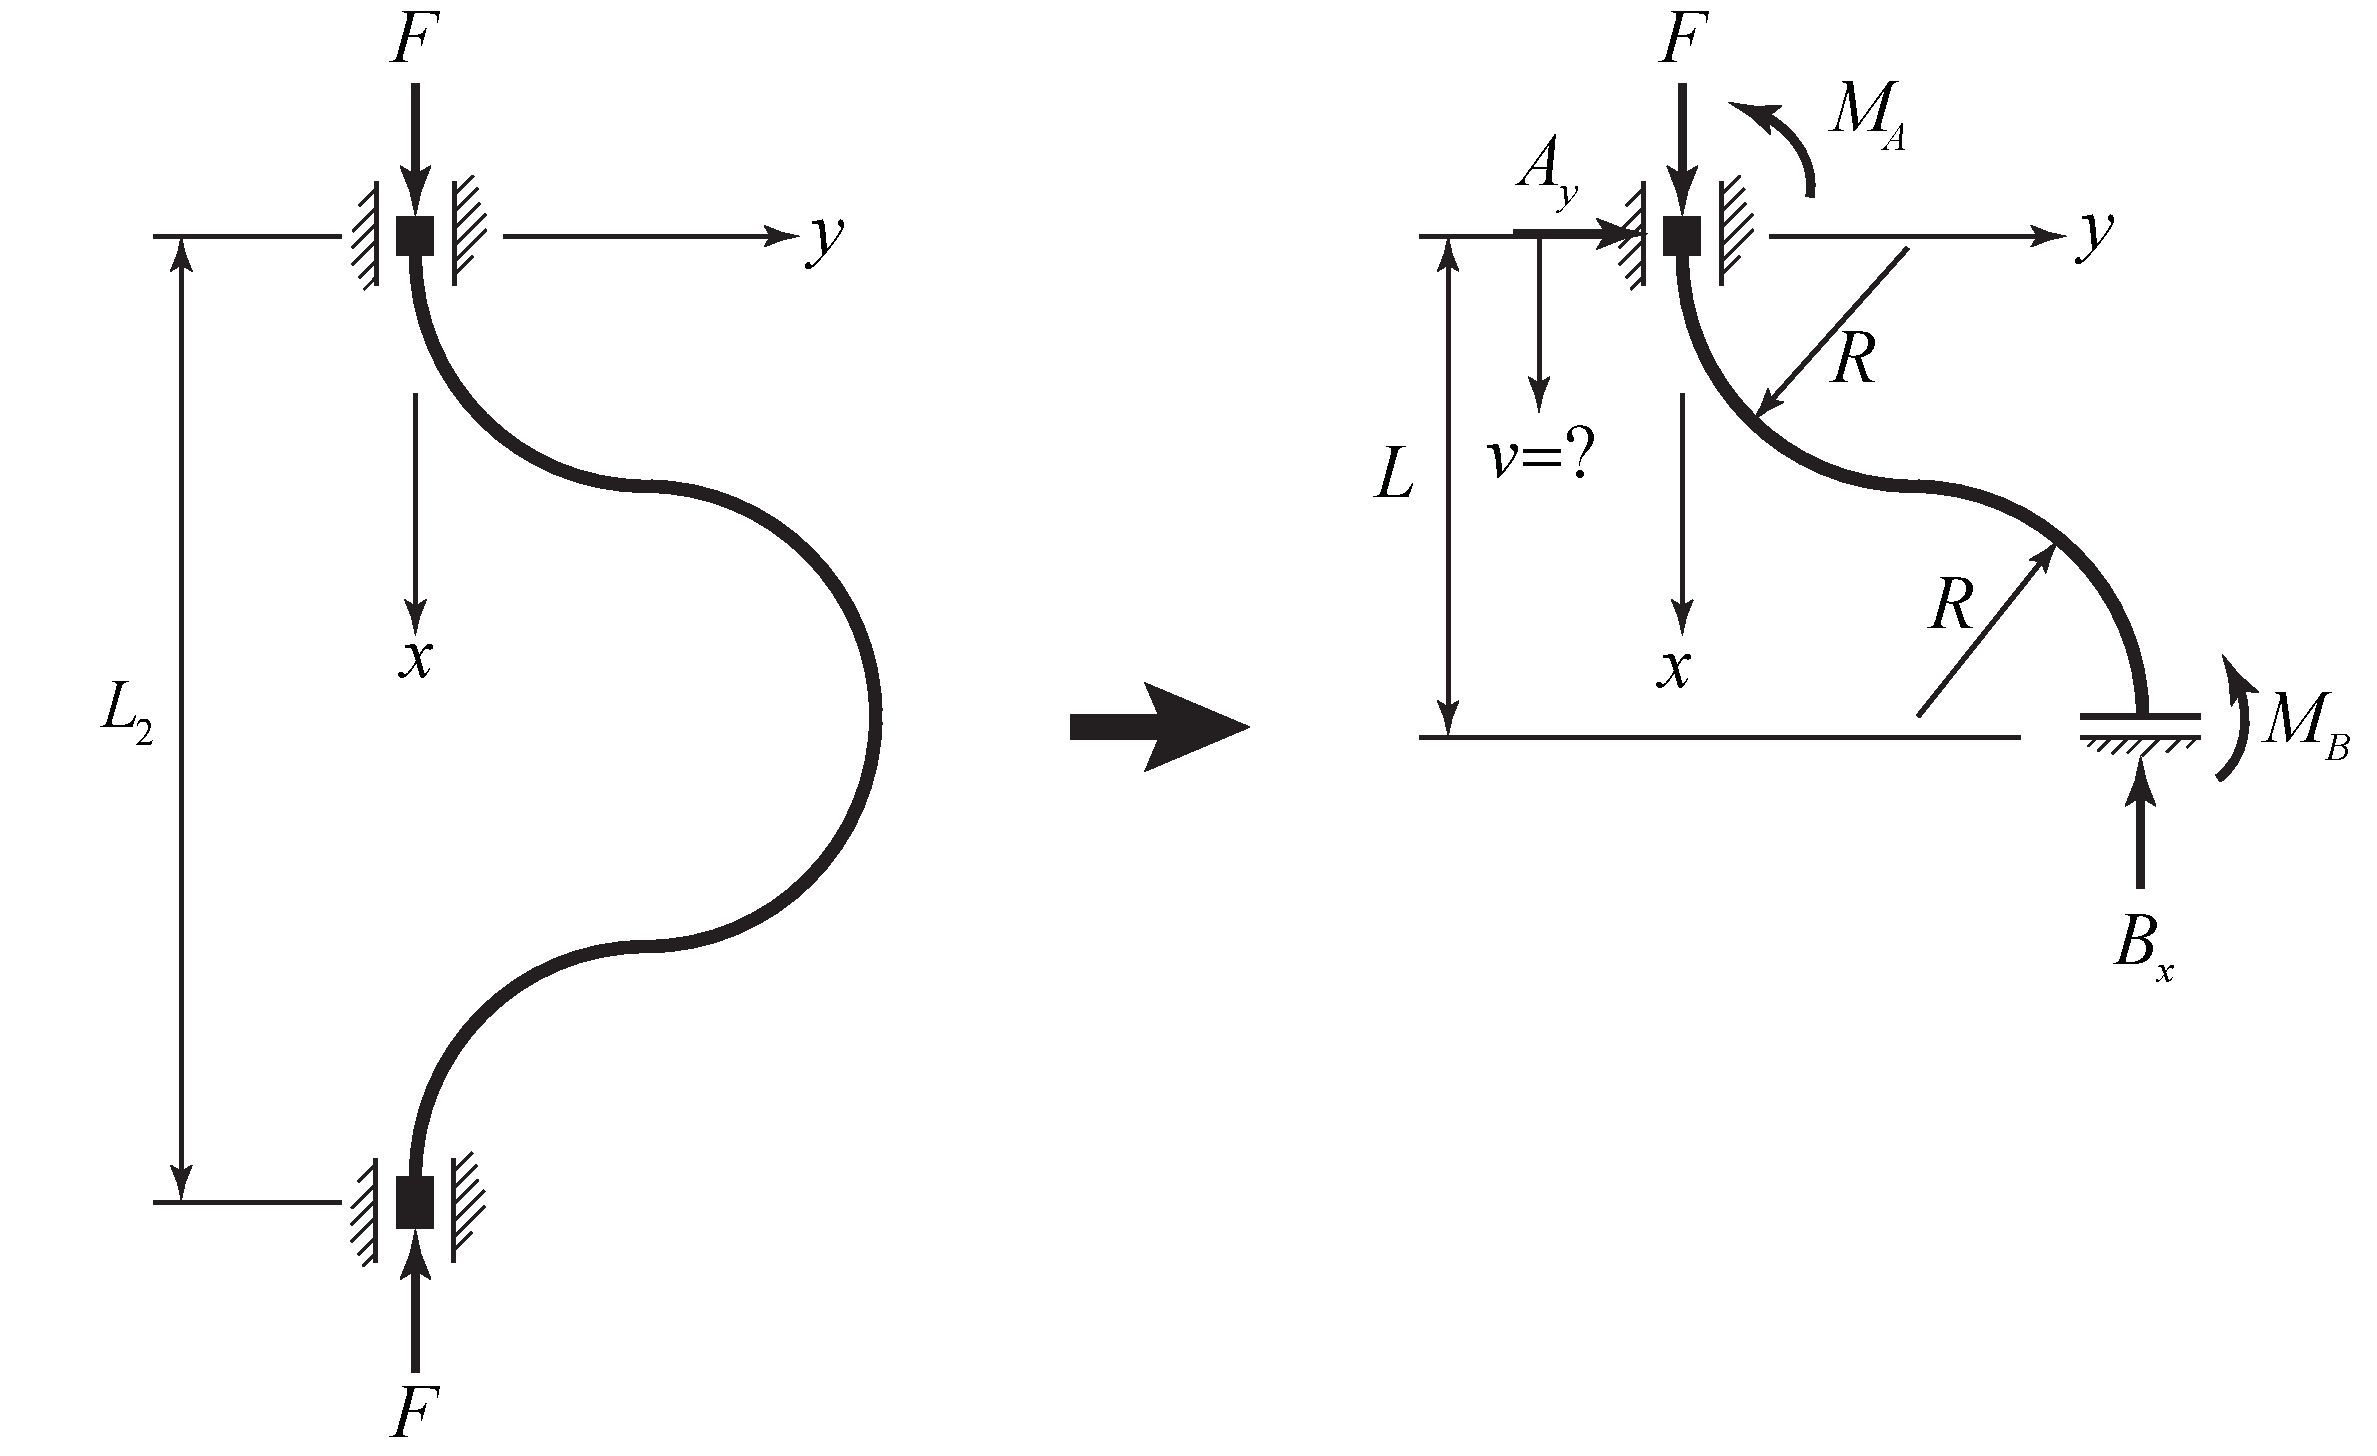
\includegraphics[scale=0.32]{Magisterski praktikum/slike/teorija/pozitivni_nosilec_poenostavitev.pdf}
                \caption{Diagram prostega telesa problema.}\label{fig:diagram prostega telesa pozitivni element}
        \end{figure}
        
        Osnovni sistem je statično nedoločen in ga razdelimo na dva določena glavna sistema, kjer je prvemu sistemu odvzeta momenta reakcija, ki se pojavi v drugem sistemu kot obremenitev (slika \ref{fig:glavni in virtualni sistemi}).
        \begin{figure}[!hb]
                \centering
                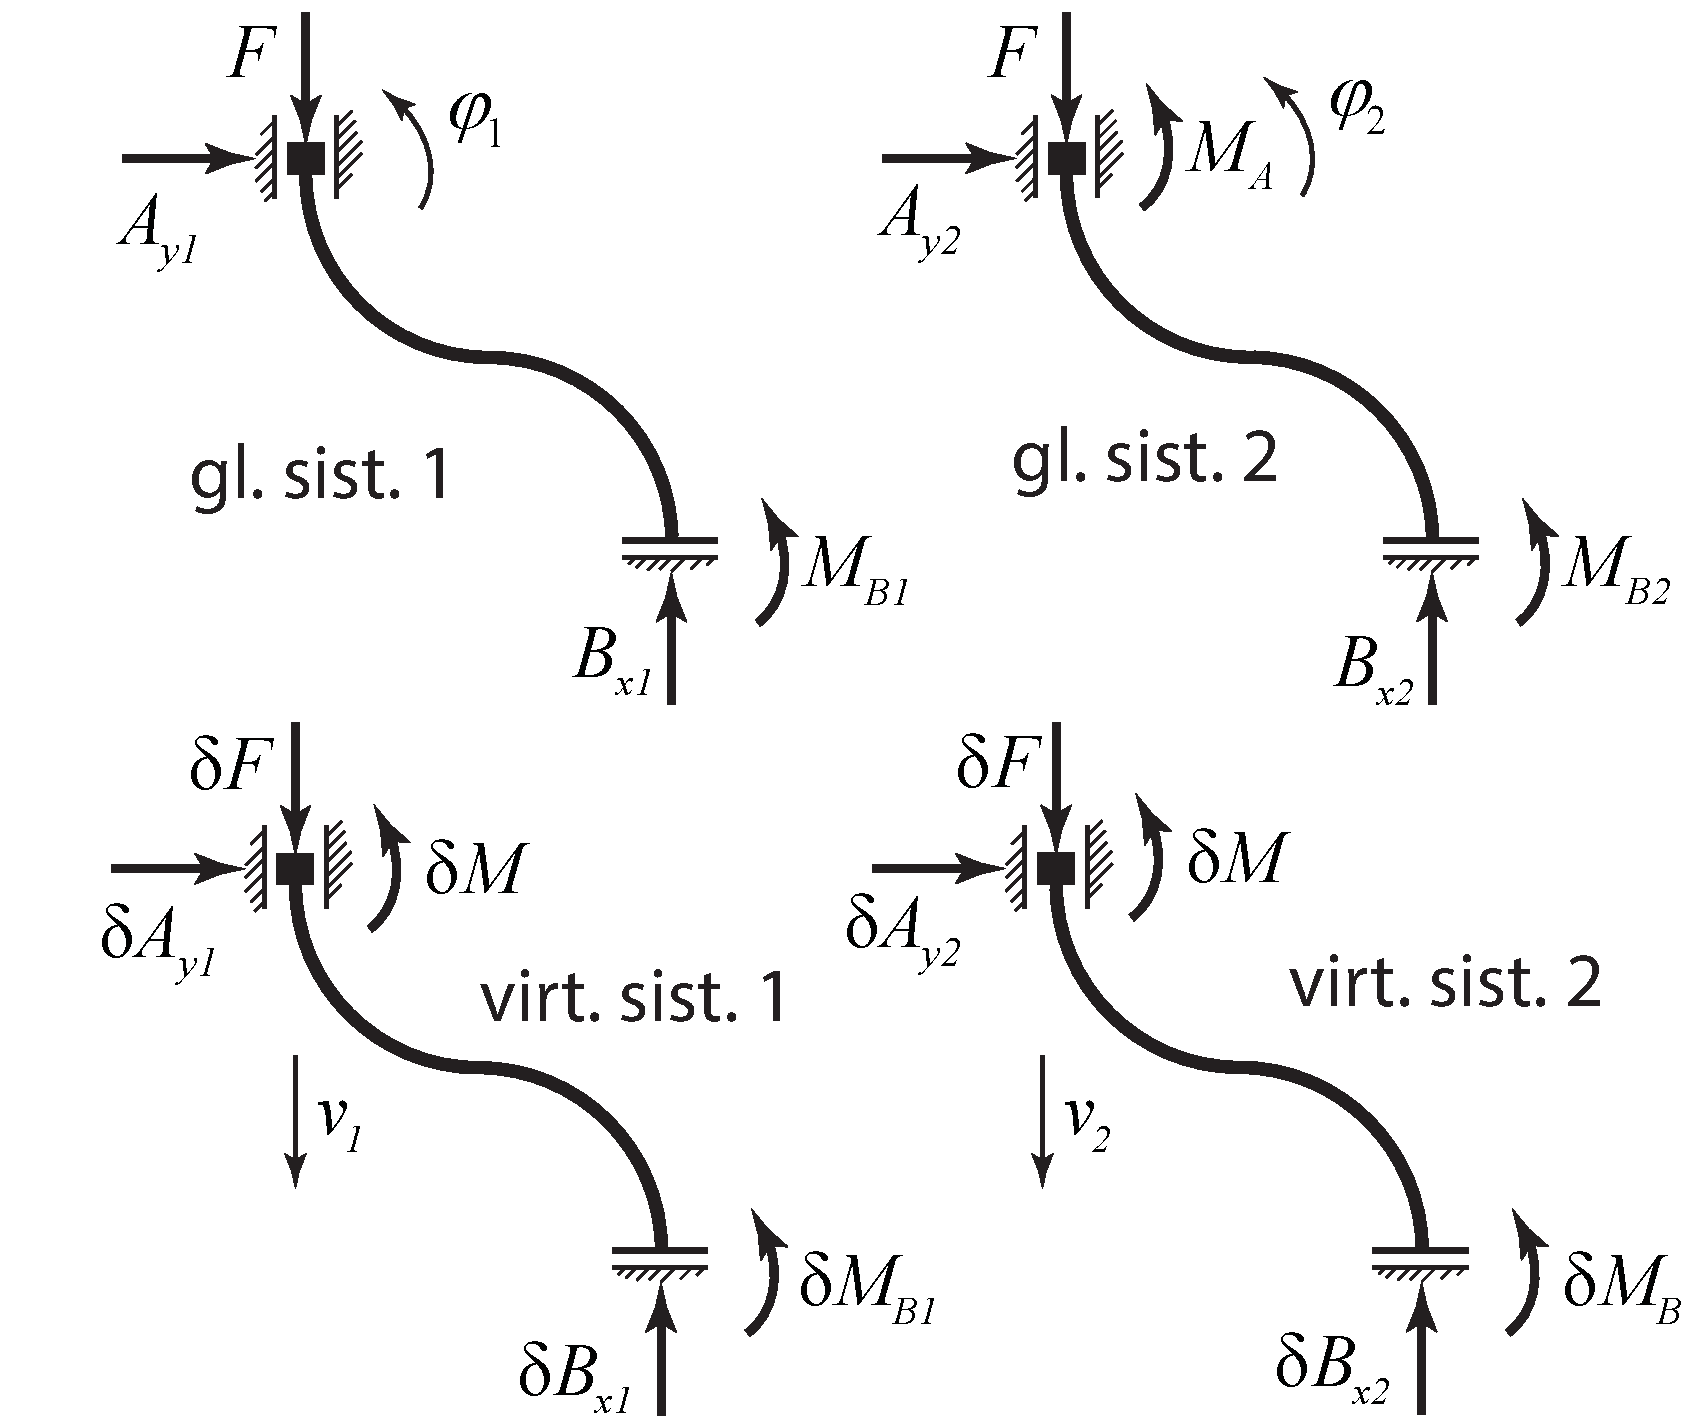
\includegraphics[scale=0.32]{Magisterski praktikum/slike/teorija/pozitivni_nosilec_sistemi.pdf}
                \caption{Glavni in virtualni sistemi.}\label{fig:glavni in virtualni sistemi}
        \end{figure}
    
    
        \newpage
        Za izračun pomika togosti $k_p$ uporabimo virtualno delo, ki je aplikacija principa najmanjše akcije - virtualno delo, ki ga opravi virtualna obremenitev, bo vedno minimalen. Vsakemu od glavnih sistemov (ločeno) pripišemo virtualne obremenitve $\delta F$ in $\delta M$. Glavna sistema imata dve polji I in II, ki jih modeliramo kot četrtino krožnice  $\varphi \in [0, \varphi/2]$. Glavni sistem 1 z obremenitvijo $F$ in glavni sistem 2 z obremenitvijo $M_\text{A}$ imata notranje momente definirane kot:
        \begin{align}
            M_{\text{I},1}(\varphi) &= -FR (1-\cos\varphi) \nonumber \\ 
            M_{\text{II},1}(\varphi) &= -FR (1+\sin\varphi) \nonumber \\ 
            M_{\text{I},2}(\varphi) &= -M_\text{A} \nonumber \\ 
            M_{\text{II},2}(\varphi) &= -M_\text{A} \,,
        \end{align}
        kjer je $R$ polmer loka nosilca.  
        
        Virtualni moment $\delta M$ povzroča rotacijo v točki A in je uporabljen za izračun neznane reakcijske sile $M_A$. Notranje obremenitve virtualnih sistemov so: 
        \begin{align}
            \delta M_{\text{I},1} = \delta M_{\text{II},1} = \delta M_{\text{I},2}= \delta M_{\text{II},2} = - \delta M \,.
        \end{align}
        
        Virtualno delo notranjih obremenitev $\delta W_\text{N}$ in zunanjih obremenitev $\delta W_\text{Z}$, zaradi $N$ sil in $K$ momentov, je po principu virtualnih sil in momentov definirano kot:
        \begin{align}
            \delta W_\text{N} &=  \int_{s}^{} \frac{M  \, \delta M}{E I} \,\text{d}s =  \int_{\varphi}^{} \frac{M  \, \delta M}{E I} R \,\text{d}\varphi \, ,\\
            \delta W_\text{Z} &=  \sum_{i=1}^{N} \delta F_i \delta v_i + \sum_{j=1}^{K} \delta M_j \delta \varphi_j    \,,
        \end{align}
        pri čemer je $E$ modul elastičnosti in $I=I_1=b \, t_1^3 /12$ vztrajnostni moment prereza. \\ $b$ je globina in $t_1$ širina nosilca. Velja: 
        \begin{align}\label{eq:virtualno delo_enakost}
             \delta W_\text{N} = \delta W_\text{Z}\,.
        \end{align}
        
        Za prvi sistem lahko izračunamo in  nato iz enakosti v enačbi \eqref{eq:virtualno delo_enakost} dobimo $\varphi_1$:
        \begin{align}
             W_{\text{N}, 1} &= \int_{0}^{\pi/2} \frac{M_{\text{I},1} \, \delta M_{\text{I},1}}{E I} R \,\text{d}s +
             \int_{0}^{\pi/2} \frac{M_{\text{II},1}  \, \delta M_{\text{II},1}}{E I} R \,\text{d}\varphi =
             \pi  \, \frac{F R^2  \, \delta M}{E I} \,, \\
             W_{\text{Z}, 1} &= \delta M \, \varphi_1 \,,  \\
             \varphi_1 &= \pi \frac{F R^2}{E I} \,.
        \end{align}
        Podobno uporabimo notranje reakcije drugega glavnega in virtualnega sistema za:
        \begin{align}
             \varphi_2 &= \pi \frac{M_A}{E I} \,.
        \end{align}

        Dejanska rotacija je zaradi toge podpore omejena in velja pogoj $\varphi_1 + \varphi_2 = 0$, kar pomeni, da je momentna reakcija v podpori enaka:
        \begin{align}
             M_\text{A}= - F R \,.
        \end{align}
        
        \newpage
        Ker nas zanima togost $k_p=\Delta F / \Delta v$, potrebujemo skrček nosilca v navpični smeri $v$, ki je posledica delovanja virtualne sile $\delta F$ v točki A. Notranje obremenitve so:
        \begin{align}
            \delta M_{\text{I},1}(\varphi) &= \delta M_{\text{I},2}(\varphi) = -\delta F (1 - \cos\varphi) \nonumber \,,\\
            \delta M_{\text{II},1}(\varphi) &= \delta M_{\text{II},2}(\varphi) = -\delta F (1 + \sin\varphi) \,.
        \end{align}
        
        Podobno kot smo že prej, uporabimo notranje reakcije prvega in drugega glavnega ter virtualnega sistema in nato preko virtualnega dela dobimo:
        \begin{align}
            v_1 &= \frac{3 \pi}{2} \frac{F R^3}{E I} \, \text{ in} \\
            v_2 &= \pi \frac{M_A \, R^2}{E I} = - \pi \frac{F R^3}{E I}  \,.
        \end{align}
        
        Navpični pomik elementa s pozitivno togostjo $v_p$ povzroči dejanska sila $F$. Upoštevamo simetrijo, superpozicijo in dolžino celotnega nosilca, ki je $l_1=4 R$. Vidimo, da je:
        \begin{align}
            v_p = 2 ( v_1 + v_2 ) = \frac{\pi}{2^6} \frac{F l_1^3}{E I_1}  \,.
        \end{align}
        
        končno togost pozitivnega elementa izračunamo kot:
        \begin{align}\label{eq:kp}
            k_p = \frac{\Delta F}{\Delta v_p} = \frac{F-0}{v_p-0} = \frac{2^6}{\pi} \frac{E I_1}{l_1^3} \approx 20,372 \, \frac{E I_1}{l_1^3}\,.
        \end{align}
        
    \section{Izpeljava elementa z negativni togostjo}\label{sec:Izpeljava_elementa_z_negativno_togostjo}
    
        Element z negativno togostjo ROC sestoji iz štirih togo vpetih kosinusnih lokov dolžine $l_2$, globine $b$, debeline $t_2$, razdaljo od poravnane lege do srednje linije loka $h$ in modul elastičnosti $E$. Izpeljimo nadomestno togost iz sledeče bistabilnostne analize \cite{liu2000microelectromech} spodnjega elementa (slika \ref{fig:kosinusni nosilec}).
        \begin{figure}[!hb]
                \centering
                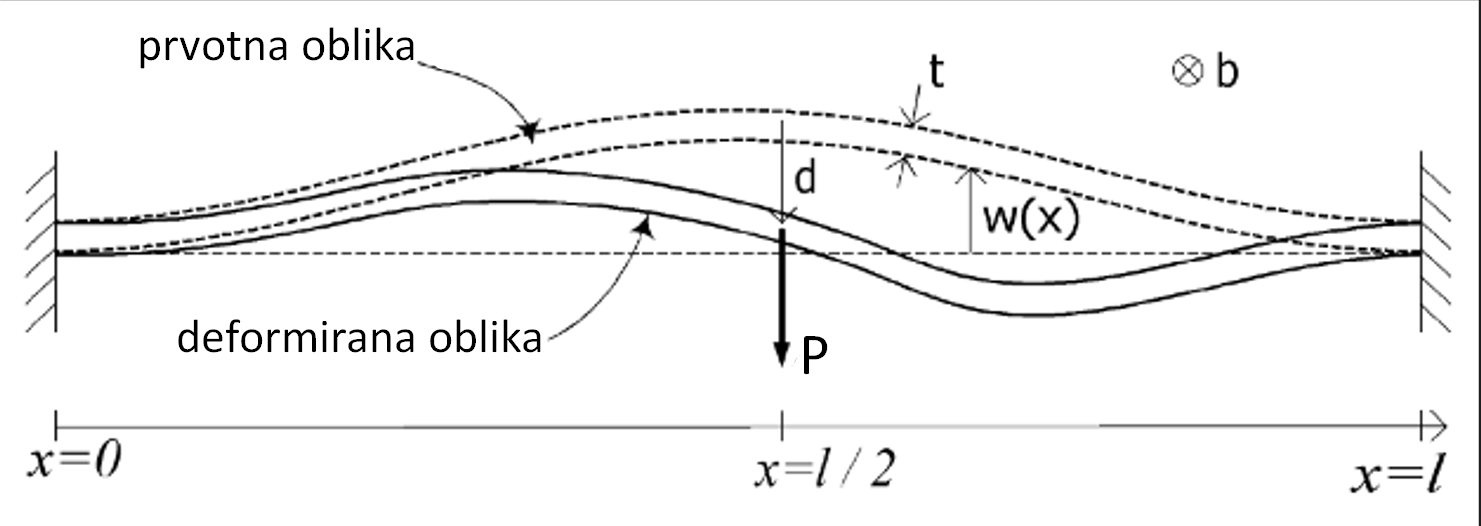
\includegraphics[trim=0 0 0.1cm 0.1cm, clip, scale=0.4]{Magisterski praktikum/slike/teorija/kosinusni nosilec.png}
                \caption{Shema kosinusnega nosilca.}\label{fig:kosinusni nosilec}
        \end{figure}
        
        \newpage
        Izhajamo iz enačbe Euler-Bernulijevega nosilca obremenjenega z aksialno silo $P$: 
        \begin{equation}
            E I_2 \frac{\dd ^4 w}{\dd x^4}+P \frac{\dd^2 w}{\dd x^2}=0 \, ,
        \end{equation}
        
        kjer je $w=w(x)$ prečni pomik nosilca. Togo vpet nosilec ima robne pogoje:
        \begin{equation}
            w(0)=w(l_2)=0, \quad\left(\frac{\dd w}{\dd x}\right)_{x=0}=\left(\frac{\dd w}{\dd x}\right)_{x=l_2}=0 \, .
        \end{equation}
        Vpeljemo definicijo normirane aksialne sile, ki je enaka:
        \begin{equation}
            N^2=\frac{P \, l_2^2}{E I_2} \, .
        \end{equation}
        
        Reševanje diferencialne enačbe vodi v pogojno enačbo:
        \begin{equation}
            \sin \left(\frac{N}{2}\right)\left[\tan \left(\frac{N}{2}\right)-\frac{N}{2}\right]=0 \,
        \end{equation}
        in dve vrsti rešitev, kjer je prva:
        \begin{equation}\label{eq:def_ob_1}
            \left.\begin{array}{l}
            w_j(x)=C\left[1-\cos \left(N_j \frac{x}{l_2}\right)\right] \\
            N_j=(j+1) \pi
            \end{array}\right\} \quad j = 1, 3, 5 \ldots
        \end{equation}
        in druga: 
        \begin{equation}\label{eq:def_obl_2}
            \begin{aligned}
            &\left.w_j(x)=C\left[1-2 \frac{x}{l_2}-\cos \left(N_j \frac{x}{l_2}\right)+\frac{2 \sin \left(N_j \frac{x}{l_2}\right)}{N_j}\right]\right\} \quad j=2, 4, 6 \ldots \\
            &N_j=2,86 \pi; \, 4,92 \pi \ldots
            \end{aligned}
        \end{equation}
        
        Zgornja analiza podaja matematično osnovo stabilnostne analize uklona nosilca. Namesto prednapetega nosilca, lahko izhajamo iz nosilca, katerega izhodišče je hkrati prva deformacijska oblika z enačbo:
        \begin{equation}
            \bar w(x)=\frac{h}{2}\left[1-\cos \left(2 \pi \frac{x}{l_2}\right)\right] \,.
        \end{equation}
        
        Ob obremenitvi nosilca z lateralno silo $F$ pri $x=l_2/2$, se središče nosilca ob predpostavki majhnih pomikov poda za $d$ in dolžina nosilca postane $s$: 
        \begin{align}\label{eq:dolzina_d}
            d &= \bar w \left(\frac{l_2}{2}\right)-w\left(\frac{l_2}{2}\right) \,, \\
            s &= \int_0^{l_2} \sqrt{1+\left(\frac{\dd w}{\dd x}\right)^2} \dd x \approx \int_0^{l_2}\left[1+\frac{1}{2}\left(\frac{\dd w}{\dd x}\right)^2\right] \dd x \,.
        \end{align}
        
        Sprememba $s$ povzroči nastanek aksialne sile: 
        \begin{equation}
            P = E \, b \, t \left(1 - \frac{s}{s_0}\right) \,,
        \end{equation}
        kjer je $s_0=l_2$ začetna dolžina nosilca. 
        
        Med deformacijo je prisotna upogibna energija $u_b$, tlačna energija $u_s$ in energija aktuacije $u_f$. Variacija energij je: 
        \begin{align}\label{eq:variacija_energij}
            \partial u_b &= \partial\left[\frac{E I}{2} \int_0^{l_2}\left(\frac{\dd^2 \bar{w}}{\dd x^2}-\frac{\dd^2 w}{\dd x^2}\right)^2 \dd x\right] \,,\\
            \partial u_s &= -P \partial s \,,\\
            \partial u_s &= -F \partial d \,.
        \end{align}
        
        Problem rešujemo s superpozicijo deformacijskih oblik. Deformacijske oblike po enačbah \eqref{eq:def_ob_1} in \eqref{eq:def_obl_2} so ortogonalne in jih lahko uporabimo tudi kot osnovo za izračun pomika $w$ prvotno deformiranega nosilca, saj so robni pogoji enaki. Sprva normiramo parameter:
        \begin{equation}
            X = \frac{x}{l_2} \,, \,\, W(X)=\frac{X l_2}{h}  \, .
        \end{equation}
        
        Torej je superpozicija oblike nosilca: 
        \begin{equation}
            W(X) = \sum_{j=1}^{\infty} A_j W_j(X) \,.
        \end{equation}
        in obe rešitvi:
        \begin{equation}
            \left.\begin{array}{l}
            W_j(X)=1-\cos \left(N_j X\right) \\
            N_j=(j+1) \pi
            \end{array}\right\} \quad j=1, 3, 5 \ldots
        \end{equation}
        \begin{equation}
            \left.\begin{array}{l}
            W_j(x)=1-2 X-\cos \left(N_j X\right)+\frac{2 \sin \left(N_j X\right)}{N_j} \\
            N_j=2,86 \pi; 1,92 \pi \ldots
            \end{array}\right\} \quad j = 2, 4, 6 \ldots
        \end{equation}
        
        Prvotna normirana oblika nosilca je: 
        \begin{equation}
            \bar{W}(X)=\frac{1}{2} W_0(X) \,.
        \end{equation}
        
        Normiramo tudi preostale parametre:
        \begin{equation}\label{eq:normalizacija}
            \begin{aligned}
            R &=\frac{F l_2^3}{E I h}, \quad \Delta=\frac{d}{h}, \quad S=\frac{s l_2}{h^2}, \quad N^2=\frac{P l_2^2}{E I}, \quad Q=\frac{h}{t_2} \\
            U_b &=\frac{u_b l_2^3}{E I h^2}, \quad U_s=\frac{u_s l_2^3}{E_j I h^2}, \quad U_f=\frac{u_f l_2^3}{E I h^2} \,.
            \end{aligned}
        \end{equation}
        
        S superpozicijo in normiranjem lahko relacije \eqref{eq:dolzina_d} do \eqref{eq:variacija_energij} izrazimo kot:
        \begin{equation}
            \begin{aligned}
            \Delta &=1-2 \sum_{j=1, 5, 9 \ldots} A_j \,, \\
            S &=1+\sum_{j=1}^{\infty} \frac{A_j^2 N_j^2}{4} \,, \\
            \frac{N^2}{12 Q^2} &=(S)_{W=\bar{W}}-S=\frac{N_1^2}{16}-\sum_{j=1}^{\infty} \frac{A_j^2 N_j^2}{4} \, ,\\
            \partial U_b &=\partial\left[\frac{\left(\frac{1}{2}-A_1\right)^2 N_1^4}{4}+\sum_{j=2}^{\infty} \frac{A_j^2 N_j^4}{4}\right] \,, \\
            \partial U_s &=-N^2 \partial S = -N^2 \partial\left(\sum_{j=1}^{\infty} \frac{A_j^2 N_j^2}{4}\right) \text{ in} \\
            \partial U_f &=-R \partial\Delta=2 R \sum_{j=1, 5, 9 \ldots} A_j \,.
            \end{aligned}
        \end{equation}
        
        Variacija celotne energije $U_t$ je vsota posameznih energij:
        \begin{equation}
            \begin{aligned}
            \partial U_t =&\left(\frac{N_1^4-N^2 N_1^2}{2} A_1-\frac{N_1^4}{4}+2 F\right) \partial\left(A_1\right) \\
            &+\sum_{j=2,3,4,6,7 \ldots}\left(\frac{N_j^4-N^2 N_j^2}{4}\right) \partial\left(A_j^2\right) \\
            &+\sum_{j=5,9,13 \ldots}\left(\frac{N_j^4-N^2 N_j^2}{2} A_j+2 F\right) \partial\left(A_j\right) \,,
            \end{aligned}
        \end{equation} 
        in mora biti minimizirana:
        \begin{equation}\label{eq:minimizacija_Ut}
            \partial U_t \geq 0 \,.
        \end{equation}
        
        Koeficienti $\partial A_j$, $j=1, 5, 9, 13, ...$ morajo biti nič, kar nam podaja:  
        \begin{align}
        &A_1=-\frac{1}{2} \frac{N_1^2}{N^2-N_1^2}+\frac{4 R}{N_1^2\left(N^2-N_1^2\right)} \, ,\\
        &A_j=\frac{4 F}{N_j^2\left(N^2-N_j^2\right)}, \quad j = 5, 9, 13 \ldots \label{eq:Aj_pogoj}
        \end{align}
        
        Enačbo \eqref{eq:minimizacija_Ut} morajo izpolnjevati tudi koeficienti $\partial A_j^2$, $j=2, 3, 4, 6, 7, ...$, ki imajo glede na pogoje vrednosti:
        \begin{equation}\label{eq:drugi_pogoj}
        A_j \begin{cases}=0, & N^2<N_j^2 \\ \text { mora biti omejen} & N^2>N_j^2 \\ \text { poljubna vrednost dokler je } j=2, 3, 4, 6, 7, ... & N^2=N_j^2 \end{cases}
        \end{equation}
        
        \newpage
        Iz praktičnih razlogov je mogoče mehansko omejiti le drugo deformacijsko obliko, ne da bi to vplivalo na prvo, zato drugi pogoj \eqref{eq:drugi_pogoj} narekuje, da lahko dobi $j$ vrednost 2, kadar druga oblika ni omejena, ali 3, kadar je druga oblike omejena. 
        
        Enačba \eqref{eq:drugi_pogoj} omogoča tri vrste rešitev. Prva je:
        \begin{equation}
            \left\{\begin{array}{l}
            R=R_1 \\
            N^2<\left\{\begin{aligned}
            N_1^2, & \text { z omejeno drugo deformacijsko obliko } \\
            N_2^2, & \text { z neomejeno drugo deformacijsko obliko }
            \end{aligned}\right. \\
            A_j=0, \quad j \neq 1, 5, 9, 13 \ldots
            \end{array}\right.
        \end{equation}
        druga:
        \begin{equation}
            \left\{\begin{array}{l}
            R=R_2 \\
            N^2=N_2^2 \\
            A_j=0, \quad j \neq 1, 2, 5, 9, 13 \ldots
            \end{array}\right.
        \end{equation}
        in tretja:
        \begin{equation}
            \left\{\begin{array}{l}
            R=R_3 \\
            N^2=N_3^2 \\
            A_j=0, \quad j \neq 1, 3, 5, 9, 13 \ldots
            \end{array}\right.
        \end{equation}
        
        Z do sedaj izpeljanimi enačbami lahko definiramo relacijo med normirano obremenitvijo  $R$ in pomikom $\Delta$ kosinusnega nosilca. Če zanemarimo višje rede $j$-ja, lahko dobimo analitične rešitve. Torej pri $A_j=0$ in $j=5, 9, 13, ...$ dobimo:
        \begin{align}
        R_1&=\frac{3 \pi^4 Q^2}{2} \Delta\left(\Delta-\frac{3}{2}+\sqrt{\frac{1}{4}-\frac{4}{3 Q^2}}\right)\left(\Delta-\frac{3}{2}-\sqrt{\frac{1}{4}-\frac{4}{3 Q^2}}\right) \\
        R_2&=\frac{N_1^2\left(N_2^2-N_1^2\right)}{8}\left(\frac{N_2^2}{N_2^2-N_1^2}-\Delta\right)=4,18 \pi^4-2,18 \pi^4 \Delta \\
        R_3&=\frac{N_1^2\left(N_3^2-N_1^2\right)}{8}\left(\frac{N_3^2}{N_3^2-N_1^2}-\Delta\right)=8 \pi^4-6 \pi^4 \Delta
        \end{align}
        
        $R_2$ obstaja, če imamo omejeno drugo obliko in če je $Q > 2 N_2/\sqrt{3}N_1=1,67$. $R_3$ obstaja, če imamo omejeno drugo obliko in če je $Q > 2 N_3/\sqrt{3}N_1=2,31$. 
        
        Z omejeno drugo deformacijsko obliko in dovolj velikim $Q > 2,31$ lahko vse tri rešitve $R$ lineariziramo. Če $R_1$,  $R_2$, $R_3$ in $\Delta$ ponovno dimenzioniramo po enačbah \eqref{eq:normalizacija}, lahko za $Q \approx 6$ dobimo vrednosti spodaj:
        \begin{equation}
            \begin{aligned}
            &F_{\text {zg }} \approx 8 \pi^4 \frac{E I_2 h}{l_2^3}, \quad F_{\text {sp }} \approx -4 \pi^4 \frac{E I_2 h}{l_2^3}, \quad d_{\text {sr }}=1,33 h \\
            &d_{\text {zg }} \approx \frac{8 t_2}{3 Q}, \quad d_{\text {sp }} \approx 2 h-\frac{8 t_2}{3 Q}, \quad d_{\text {k }} \approx 2 h-\frac{4 t_2}{3 Q} \,.
            \end{aligned}
        \end{equation}
        
        \newpage
        Analitična rešitev je le aproksimacija, saj smo zanemarili višje člene enačbe \eqref{eq:Aj_pogoj}. Z upoštevanjem višjih redov enačbe, bi dobili boljšo aproksimacijo togosti. Dodatno upoštevamo še dva člena:
        \begin{align}
            \sum_{j=1,5,9,13 \ldots} \frac{4\left(N^2-N_1^2\right)^2}{N_j^2\left(N^2-N_j^2\right)^2} F_1^2
            -N_1^2 F_1 + \frac{N^2\left(N^2-N_1^2\right)^2}{12 Q^2}-\frac{N_1^2 N^2\left(N^2-2 N_1^2\right)}{16}=0 \,,
        \end{align}
        
        kar vodi v parametre $F$-$d$ krivulje za $Q \approx 6$, ki so grafično prikazani na sliki \ref{fig:F-d_graf} :
        \begin{equation}\label{eq:bistabilnostne_en_1}
            \begin{aligned}
            &F_{\text {zg }} \approx 740 \frac{E I_2 h}{l_2^3}, \quad F_{\text {sp }} \approx -370 \frac{E I_2 h}{l_2^3}, \quad d_{\text {sr }}=1,33 h \\
            &d_{\text {zg }} \approx 0,16 h, \quad d_{\text {sp }} \approx 1,92 h, \quad d_{\text {k }} \approx 1,99 h \,.
            \end{aligned}
        \end{equation}
        
        
        
        
        Strukturna energija v ukrivljenem nosilcu med deformacijo vsebuje upogibno in tlačno energijo. Z vidika energije se upogibna energija v nosilcu monotono povečuje, kadar koli se nosilec premika navzdol; medtem ko se tlačna energija poveča do maksimuma pred preskokom na drugo stran. Če je nosilec zasnovan tako, da je zmanjšanje tlačne energije po prečkanju sredinske črte hitrejše od povečanja energije upogibanja, nastane negativna sila, kar kaže na bistabilnost. 
        
        Na podlagi zgoraj zapisanega, je kosinusni nosilec bistabilen, če sta izpolnjena dva pogoja:
        \begin{enumerate}
          \item $Q$ (razmerje med višino vrha nosilca in njegovo debelino) mora biti dovolj velik,
          \item druga deformacijska oblika mora biti omejena.
        \end{enumerate}
        
        Pogoje lahko izpolnimo tako, da uporabimo strukturo z dvojnim kosinusnim nosilcem, ki ima med obema nosilcema togo povezavo. Središčna povezava prenaša rotacijo enega od središč nosilcev na osno gibanje drugega nosilca. Ker sta nosilca toga v aksialni smeri, se lahko rotacijsko gibanje obeh nosilcev močno zmanjša. Monostabilni mehanizem z enim nosilcem prikazan na sliki \ref{fig:enojni_nosilec}, medtem ko je bistabilni dvojni ukrivljeni nosilci so prikazani na sliki \ref{fig:dvojni_nosilec}. 
        \begin{figure}[!htb]
                \centering
                \begin{subfigure}{.489\textwidth}
                    \centering
                    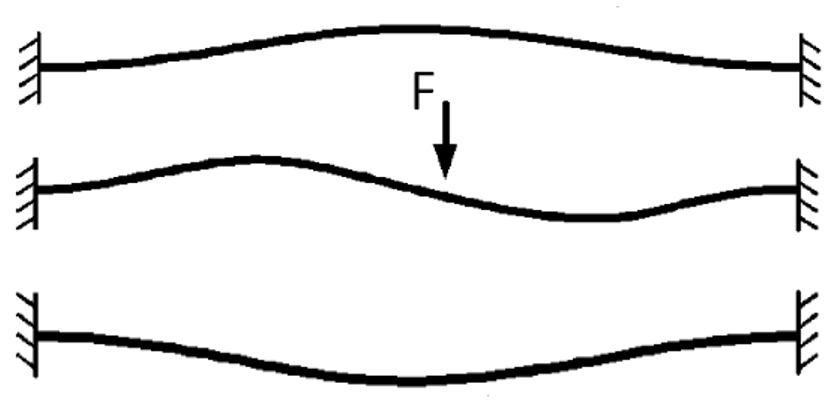
\includegraphics[width=\linewidth]{Magisterski praktikum/slike/teorija/enojni_nosilec.png}
                    \caption{}
                    \label{fig:enojni_nosilec}
                \end{subfigure}%
                \begin{subfigure}{.489\textwidth}
                    \centering
                    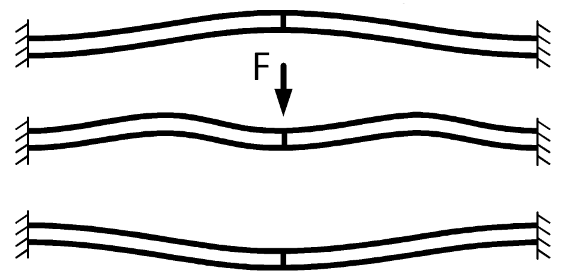
\includegraphics[width=\linewidth]{Magisterski praktikum/slike/teorija/dvojni_nosilec.png}
                    \caption{}
                    \label{fig:dvojni_nosilec}
                \end{subfigure}%
                \caption{(a) Monostabilna in (b) bistabilna konstrukcija iz nosilcev.}
                \label{fig:deformacijske_oblike}
        \end{figure}
        
        \newpage
        Krivulja $F$-$d$ dvojnega ukrivljenega nosilca bi bila videti tako, kot je prikazano na sliki  \ref{fig:F-d_graf}, pri čemer so vrednosti pomikov enake, vrednosti sile pa podvojene glede na vrednosti v enačbah \eqref{eq:bistabilnostne_en_1}: 
        \begin{equation}
            \begin{aligned}
            &F_{\text {zg }} \approx 1480 \frac{E I_2 h}{l_2^3}, \quad F_{\text {sp }} \approx -740 \frac{E I_2 h}{l_2^3}, \quad d_{\text {sr }}=1,33 h \\
            &d_{\text {zg }} \approx 0,16 h, \quad d_{\text {sp }} \approx 1,92 h, \quad d_{\text {k }} \approx 1,99 h \,.
            \end{aligned}
        \end{equation}
        
        Z $F$-$d$ diagrama \ref{fig:F-d_graf} so iz naklona premic razvidna tri področja linearne togosti. Prva nadomestna togost je $k_{n1}$, druga je iskana negativna togost $k_{n2}$, saj dosežemo negativne sile, in tretja je $k_{n3}$. 
        
        Izpeljane togosti so:
        \begin{equation}\label{eq:kn}
            \begin{gathered}
            k_{n 1}=9250 \frac{E I_2}{l_2^3}, \quad k_{n 2}=-1253,18 \frac{E I_2}{l_2^3} \text{ in} \quad k_{n 3}=10571,42 \frac{E I_2}{l_2^3}\,.
            \end{gathered}
        \end{equation}
        
        V $F$-$d$ diagram vrišemo tudi v poglavju \ref{sec:Izpeljava_elementa_s_pozitivno_togostjo} izpeljano togost $k_p$. V sledečem poglavju združimo elemente pozitivne in negativne togosti in tvorimo KNT ROC.
        

        \begin{figure}[!htb]
                \centering
                \begin{subfigure}{.489\textwidth}
                    \centering
                    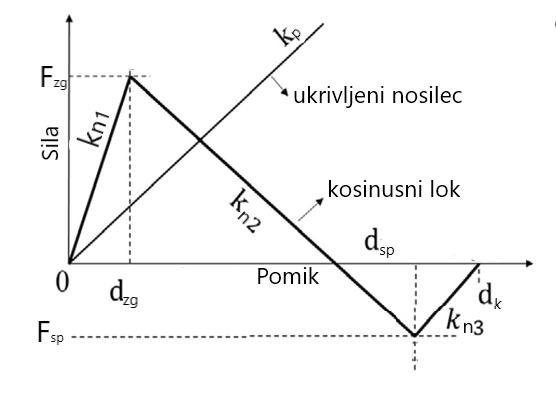
\includegraphics[trim=0 0 0 -2cm, clip, width=\linewidth]{Magisterski praktikum/slike/teorija/F-d_graf.png}
                    \caption{}
                    \label{fig:F-d_graf}
                \end{subfigure}%
                \begin{subfigure}{.489\textwidth}
                    \centering
                    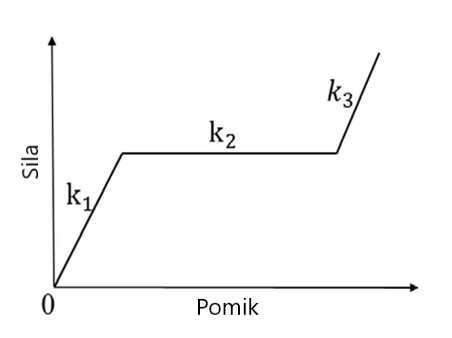
\includegraphics[trim=0 0 0 -2cm, clip, width=\linewidth]{Magisterski praktikum/slike/teorija/F-d_graf2.png}
                    \caption{}
                    \label{fig:F-d_graf2}
                \end{subfigure}%
                \caption{(a) $F$-$d$ graf pozitivnega in negativnega nosilca in (b) celotne ROC.}
        \end{figure}
        
    
    \newpage
    \section{Statična analiza ROC}\label{sec:staticna_analiza_ROC}
        
        Ker imamo z bistabilnim kosinusnim nosilcem negativne togosti (poglavje \ref{sec:Izpeljava_elementa_z_negativno_togostjo}) paralelno povezana dva nosilca pozitivne togosti (\ref{sec:Izpeljava_elementa_s_pozitivno_togostjo}), ter nato ta sistem zaporedno povezan z enakim sistemom, lahko posamezne nadomestne togosti seštejemo v: 
        \begin{equation}\label{eq:k1k2k3}
            k_1=\frac{1}{2} ( k_{n 1}+2 k_p ), \quad k_2=\frac{1}{2} ( k_{n 2}+2 k_p ) \text{ in} \quad k_3=\frac{1}{2} ( k_{n 3}+2 k_p ) \,.
        \end{equation}
        
        Na tem mestu lahko upoštevamo prej zastavljeni pogoj za KNT \eqref{eq:pogoh_KNT} in za $k_2=0$ določimo to območje kot območje ničelne togosti. Torej ob stiskanju ROC v vertikalni smeri (slika \ref{fig:shema_roc}) na začetku potrebujemo vedno večjo silo $F$. Na neki točki ob pravilno dimenzioniranih nosilcih, za nadaljnjo pomikanje, sila ostaja enaka. To je zaradi negativne togosti $k_{n2}$, ki deluje z nasprotujočo silo. Ko nekaj časa pomikamo ROC, ponovno preidemo v območje pozitivne togosti in potrebna sila se spet poveča. V vmesnem področju imamo prisotno KNT. Na sliki \ref{fig:referencni_sistem} vidimo sistem vzmeti z maso, ki jo uporabimo kot referenco za izpeljavo povezave med razmerjem togosti $\mu$ in geometrijskega parametra $\gamma$, ki ju uporabimo za dimenzioniranje nosilcev \cite{dalela2022design}. 
        \begin{figure}[!htb]
                \centering
                \begin{subfigure}{.341\textwidth}
                    \centering
                    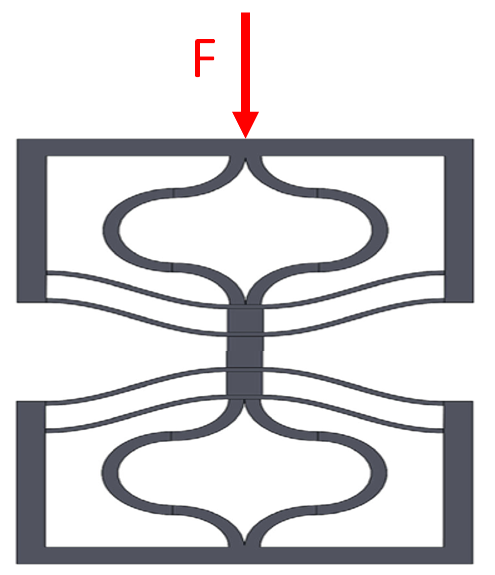
\includegraphics[width=\linewidth]{Magisterski praktikum/slike/teorija/shema_ROC.png}
                    \caption{}
                    \label{fig:shema_roc}
                \end{subfigure}%
                \begin{subfigure}{.341\textwidth}
                    \centering
                    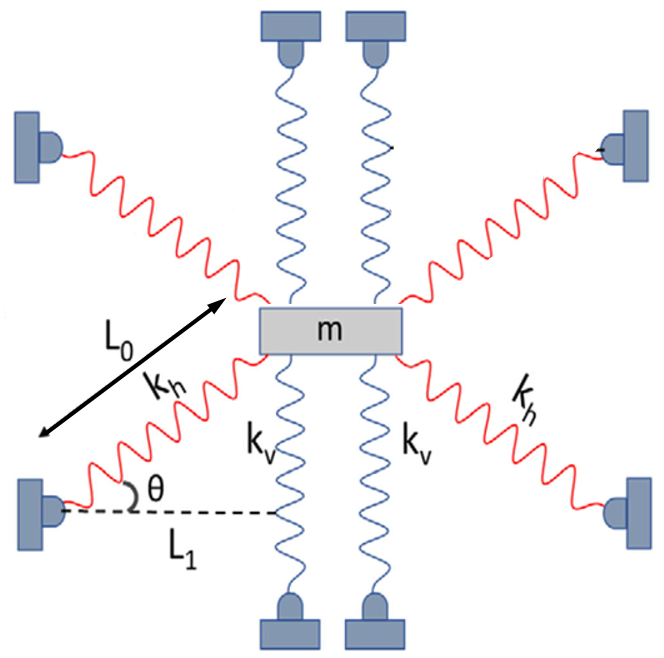
\includegraphics[width=\linewidth]{Magisterski praktikum/slike/teorija/referencni_sistem.png}
                    \caption{}
                    \label{fig:referencni_sistem}
                \end{subfigure}%
                \caption{(a) Shema ROC in (b) referenčni sistem z maso in vzmetjo.}
        \end{figure}
        
        Navpični nosilci za pozitivno togost imajo enako togost kot vertikalne vzmeti: 
        \begin{equation}
            k_v = k_p \,.
        \end{equation}
        
        Dvojna bistabilna kosinusna nosilca sta z horizontalno vzmetjo povezana preko relacije:
        \begin{equation}
            k_h \sin \theta=k_{n 2} \,,
        \end{equation}
        
        kjer predpostavimo, da je vertikalna komponenta ekvivalentne togosti horizontalne vzmeti enaka $k_{n 2}$. Ko ROC doživi vertikalni pomik $d$ iz statične ravnovesne lege, vsaka polovica doživi pomik $X=d/2$ in je sila kosinusnega nosilca:
        \begin{equation}\label{eq:F_h}
            F_h=k_h\left(L_0-\sqrt{L_1^2+X^2}\right)\,.
        \end{equation}
        
        Tukaj je $L_0$ prvotna razdalja od roba nosilca do njegove sredine in $L_1$ horizontalna razdalja od roba do sredine. Vertikalna komponenta kosinusnega sile nosilca $F_{\mathrm{MNT}}$, ki služi kot mehanizem negativne togosti (MNT), je:
        \begin{equation}\label{eq:F_MNT}
            F_{\mathrm{MNT}}=-F_h \sin \theta = - F_{h} \frac{X}{\sqrt{L_1^2+X^2}}\,,
        \end{equation}
        s kotom med kosinusnim nosilcem in horizontalno ravnino $\theta$.
        
        Za ROC je relacija sila-pomik: 
        \begin{equation}
            F_v= k_v X 
        \end{equation}
        in relacija za MNT, pridobljena z združitvijo enačb \eqref{eq:F_h} in \eqref{eq:F_MNT}, je:
        \begin{equation}
            F_{\mathrm{MNT}}(X)=-\frac{1}{2} k_h\left(\frac{L_0}{\sqrt{L_1^2+X^2}}-1\right) X \,.
        \end{equation}
        
        Za zasnovano ROC je odvisnost sile od pomika:
        \begin{equation}\label{eq:F-ROC}
            \begin{aligned}
            F_{\mathrm{ROC}}(X)&=F_v+F_{\mathrm{MNT}}(X) \,\\
            F_{\mathrm{ROC}}(X)&= k_v X-\frac{1}{2} k_h\left(\frac{L_0}{\sqrt{L_1^2+X^2}}-1\right) X\,.
            \end{aligned}
        \end{equation}
        
        Zgornjo enačbo lahko zapišemo v brezdimenzijski obliki z vpeljavo:
        \begin{equation}
            f_{\mathrm{ROC}}(x)=\frac{F_{\mathrm{ROC}}(X)}{k_v L_0}, \quad \mu=\frac{k_h}{k_v}, \quad \gamma=\frac{L_1}{L_0}, \quad x=\frac{X}{L_0} \,.
        \end{equation}
        
        Tako lahko zapišemo brezdimenzijsko enačbo ROC na sliki \ref{fig:shema_roc}, ki je:
        \begin{equation}\label{eq:brezdimenzijski_f(x)}
            f_{\mathrm{ROC}}(x)= x- \frac{1}{2} \mu\left(\frac{1}{\sqrt{\gamma^2+x^2}}-1\right) x \,.
        \end{equation}
        
        Brezdimenzijsko odvisnost togosti in pomika dobimo z odvajanjem $f_{\mathrm{ROC}}(x)$: 
        \begin{equation}
            k_{\mathrm{ROC}}(x)=1 + \frac{1}{2} \mu - \frac{2 \mu \gamma^2}{(\gamma^2+x^2)^{3/2}}\,.
        \end{equation}
        
        Togost je najmanjša v ravnovesni legi $x=0$. Za pridobitev karakteristike $KNT$ izpeljemo za $k_{\mathrm{KNT}}=k_{\mathrm{ROC}}(x=0)=0$ pogojno razmerje $\mu_{\mathrm{KNT}}$ in $\gamma_{\mathrm{KNT}}$:
        \begin{align}
            k_{\mathrm{ROC}}(0)&=1+\frac{1}{2} \mu\left(1-\frac{1}{\gamma}\right)=0 \,, \\
            \mu_{\mathrm{KNT}}&=\frac{2 \gamma}{1-\gamma} \label{eq:KNT_pogoj_1} \,, \\  
            \gamma_{\mathrm{KNT}}&=\frac{\mu}{\mu+2} \label{eq:KNT_pogoj_2} \,.
        \end{align}
        
        Jasno je, da je togost v statičnem ravnovesju negativna in nestabilna, če je vrednost $\mu > \mu_{\mathrm{KNT}}$ ali $\gamma < \gamma_{\mathrm{KNT}}$. Za namene stabilne izolacije je bolje doseči pozitivno togost v ravnovesnem položaju z izbiro parametrov na podlagi pogojev $\mu < \mu_{\mathrm{KNT}}$ ali $\gamma > \gamma_{\mathrm{KNT}}$. 
        
        Brezdimenzijska sila kot funkcija brezdimenzijskega pomika v enačbi \eqref{eq:brezdimenzijski_f(x)}, je prikazana na sliki \ref{fig:f(x)} za različne vrednosti $\gamma$ pri $\mu=\mu_{\mathrm{KNT}}$. Območje KNT je opazno, ko vrednost $f_{\mathrm{ROC}}$ ostane enaka nič pri spreminjajočem $x$. Območje KNT se povečuje s $\gamma$. Prav tako prikažemo  brezdimenzijsko karakteristiko togosti in pomika $k_{\mathrm{ROC}}(x)$, ki je prikazana na sliki \ref{fig:k(x)}. S slike vidimo, da je v položaju statičnega ravnovesja $x=0$ negativna togost, ki jo dobimo s kosinusnimi nosilci, popolnoma uravnotežena s pozitivno togostjo, tako da je kombinirana togost enaka nič.
        
        \begin{figure}[!htb]
                \centering
                \begin{subfigure}{.500\textwidth}
                    \centering
                    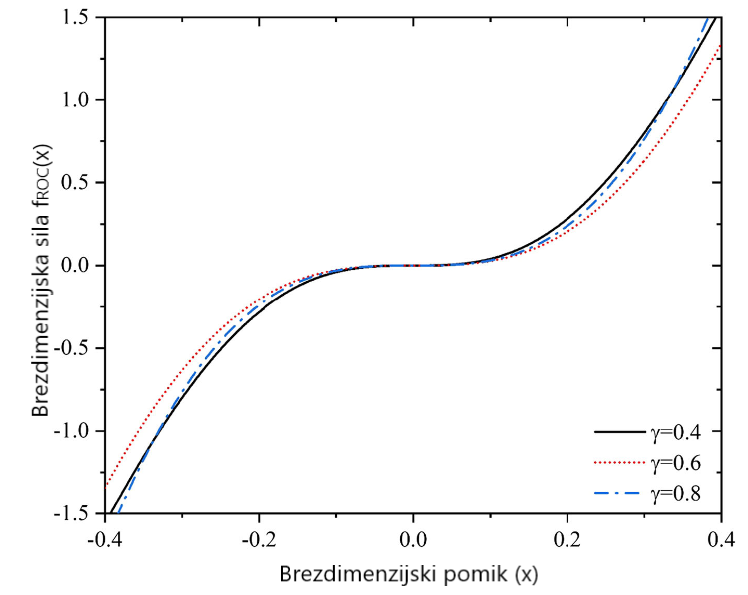
\includegraphics[width=\linewidth]{Magisterski praktikum/slike/teorija/f(x).png}
                    \caption{}
                    \label{fig:f(x)}
                \end{subfigure}%
                \begin{subfigure}{.500\textwidth}
                    \centering
                    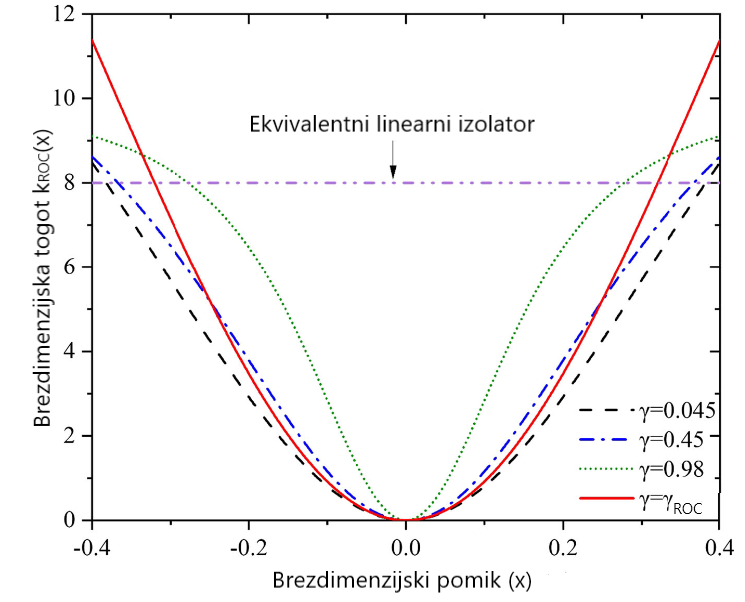
\includegraphics[width=\linewidth]{Magisterski praktikum/slike/teorija/k(x).png}
                    \caption{}
                    \label{fig:k(x)}
                \end{subfigure}%
                \caption{(a) brezdimenzijska sila in (b) togost z variiranjem $\gamma$.}
        \end{figure}

        Iz krivulje togosti in pomika, prikazane na sliki \ref{fig:k(x)}, je razvidno, da je za določeno območje pomika v odvisnosti od $\mu$ vrednost togosti KNT izolatorja manjša od vrednosti ekvivalentnega linearnega izolatorja. Območje pomikov, ki izpolnjuje nižjo vrednost togosti KNT izolatorja, je pomemben pokazatelj značilnosti togosti in pomikov in ga lahko izračunamo tako, da nastavimo vrednost togosti KNT izolatorja za manjšo od vrednosti ekvivalentnega linearnega izolatorja $k_{\mathrm{KNT}}(x)<1$. V definiciji za $k_{\mathrm{KNT}}(x)$ upoštevamo $\mu=\mu_{\mathrm{KNT}}=2\gamma/1-\gamma$ in dobimo:
        \begin{align}
            |x|&<\gamma^{2 / 3} \sqrt{1-\gamma^{2 / 3}} \,, \\
            L_{\mathrm{sd}}&=2 x=2 \gamma^{2 / 3} \sqrt{1-\gamma^{2 / 3}} \,,
        \end{align}
        
        kjer je $L_\mathrm{sd}$ dolžina pomika z nizko togostjo.  Največjo vrednost $L_\mathrm{sd}$ lahko dobimo z odvajanjem zgornje enačbe glede na $\gamma$ in izenačitvijo z ničlo. Rešitev kaže, da je $L_\mathrm{sd}$ največja pri $\gamma = 0,5443$:
        \begin{equation}
        \   L_{\mathrm{sd}}(\gamma=0,5443)=0,7698\,.
        \end{equation}
        
        
        
        
    
        
        
        
    